\normaltrue \difficilefalse \tdifficilefalse
\correctionfalse

%\UPSTIidClasse{11} % 11 sup, 12 spé
%\newcommand{\UPSTIidClasse}{11}

\exer{Diagramme de Bode $\star$ \label{C2:02:510}}
\setcounter{numques}{0}
\UPSTIcompetence[2]{C2-02}
\index{Compétence C2-02}
\index{Diagramme de Bode}
\ifcorrection
\else
\textbf{Pas de corrigé pour cet exercice.}
\fi


\ifprof 
\else
 \fi
 
\question{Tracer le diagramme de Bode de la fonction de transfert suivante : $F_1(p)=\dfrac{200}{p\left(1+20p+100p^2\right)}$.}
\ifprof
On a $\dfrac{1}{\omega_0^2} = {100}$ et $\omega_0 = \SI{0,1}{rad.s^{-1}}$.

On a $\dfrac{2\xi}{\omega_0}= {20}$ soit $\xi = \dfrac{20\times \omega_0}{2 }= 1$.

(On a donc une racine double et on pourrait remarquer que : 
$F_1(p)=\dfrac{200}{p\left(1+10p\right)^2}$).

\begin{center}
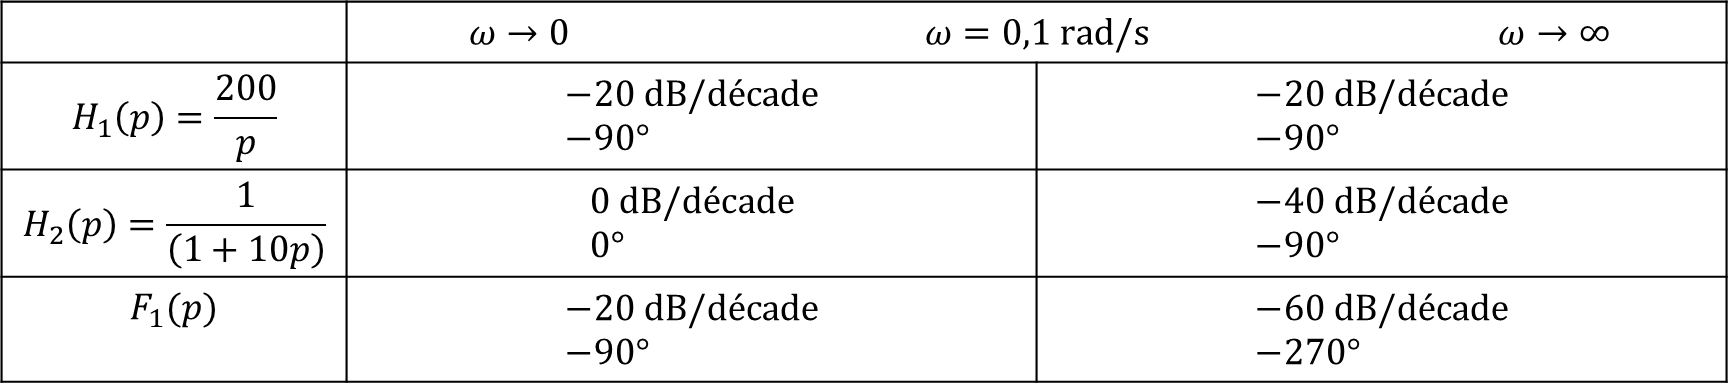
\includegraphics[width=8cm]{511_01_cor}
\end{center}

Lorsque $\omega << 0,1$, $F_1(p) \simeq \dfrac{200}{p}$ et $G_{\text{dB}}(0,1) = 20\log 200 - 20 \log 0,1 = \SI{66}{dB}$.
\begin{center}
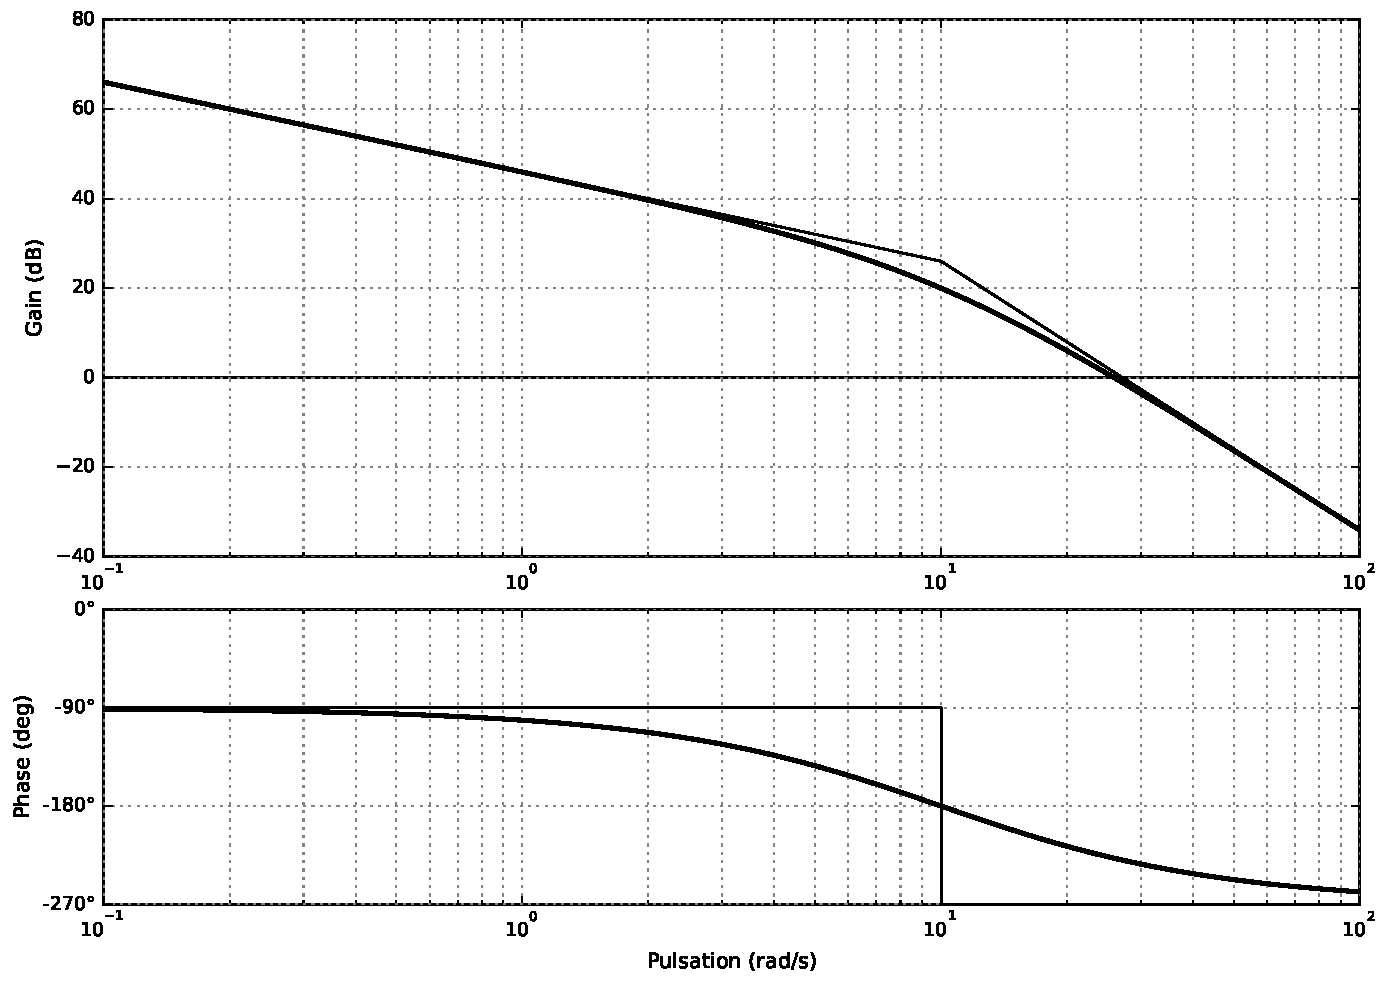
\includegraphics[width=8cm]{511_02_cor}
\end{center}

\else 
\begin{center}
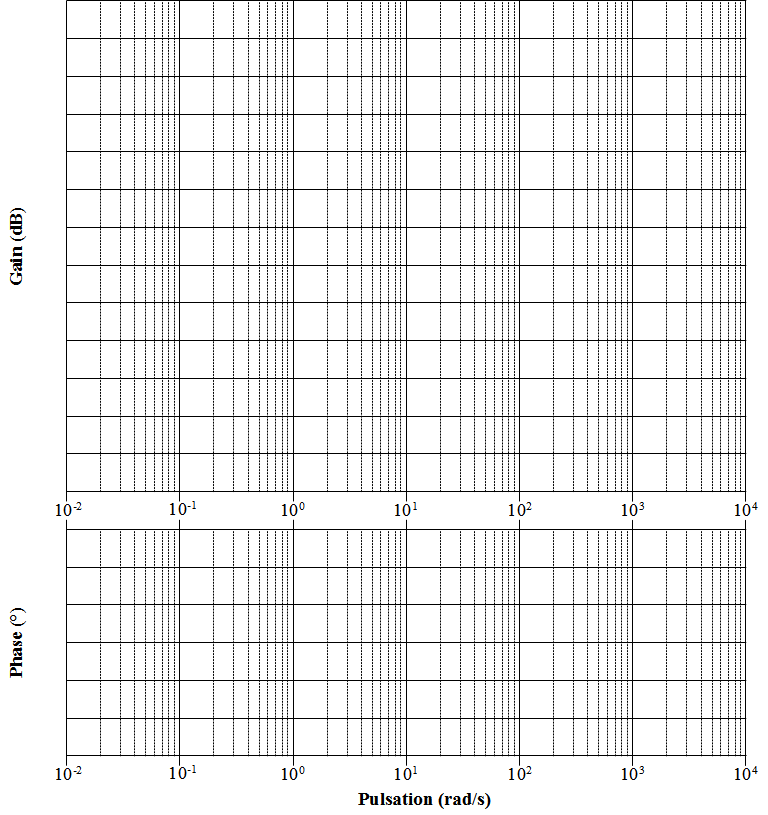
\includegraphics[width=.9\linewidth]{511_01}
\end{center}
\fi




%\question{Réaliser le schéma-blocs.}
%\ifprof
%\begin{figure}[H]
%\centering
%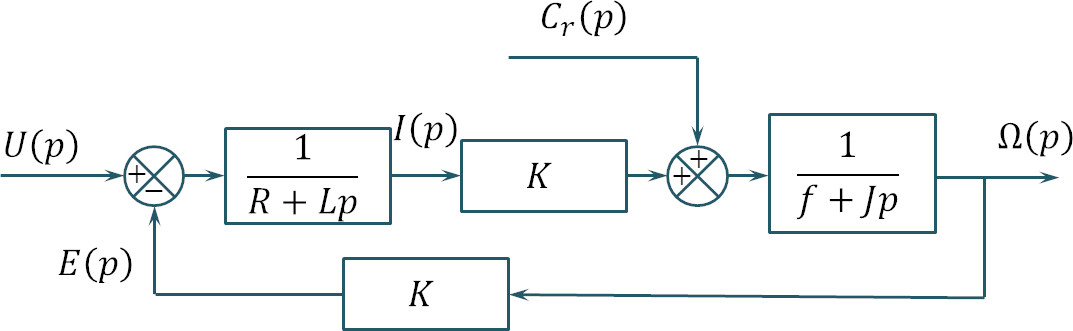
\includegraphics[width=\linewidth]{51_01_c}
%%\caption{Évolution du couple utile en fonction de la vitesse de rotation pour des
%%fréquences de commande de \SI{90}{Hz} à \SI{110}{Hz}. \label{fig_50_04}}
%\end{figure}
%\else
%\fi


 

\ifprof
\else
\begin{flushright}
\footnotesize{Corrigé  voir \ref{C2:02:510}.}
\end{flushright}%
\fi